\chapter{Topic Modeling}

In Chapter \ref{wordemb}, we presented some techniques to encode words as vectors.
Starting from a bag-of-words model in which we assume that the order of the words
inside a text does not matter, it is possible to follow a similar approach also for documents.

The first step is to generate a matrix of term counts $X$ for the entire corpus:
each row is a document represented in the BOW format and each column represents the count of occurrence
of a particular term in the documents.

The goal of the second step is to produce two matrices:
\begin{itemize}
    \item term-topic matrix: each row represents how related each term is to all topics
    \item document-topic matrix: each row represents how related each document is to all topics
\end{itemize}

For instance, a document about bears is likely to have high intensity on some topics which in turn have high
intensity on words related to animals; see Figure \ref{fig:topicmat} for an example.

\section{Latent Semantic Analysis (LSA)}
Given the number of topics $V$ as an hyperparameter,
Truncated SVD is applied to the matrix obtained in the first step
(see Figure \ref{fig:svd} for a graphical representation):
$$X_{N \times K} = U_{N \times V} \Sigma_{V \times V} D_{K \times V}^T$$

The matrix $U$ is then used as the document-topic matrix,
while $D$ represents the term-topic matrix.

Using $U$ instead of $X$ for comparing documents when $V \ll K$ leads to a smaller memory footprint.
Furthermore, the terms are no longer orthogonal: thanks to this it is possible to compute the similarity between
a term and a document even if the document does not contain the term itself.
The key point to observe is that both terms and documents are described as topics: if a term is frequent in some topics and
a document is frequent in the same topics, they will have a similar representation in the new space.

An overview of this technique can be found at \cite{doi:10.1002/aris.1440380105}.

\begin{figure}[h]
    \centering
    \subfigure{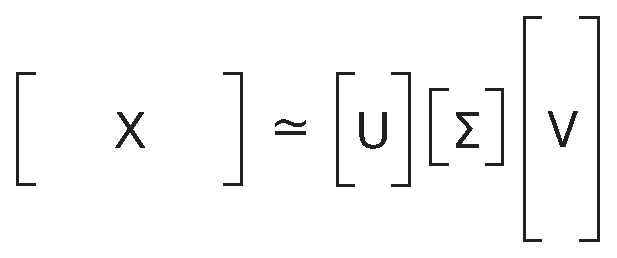
\includegraphics[width=0.5\textwidth]{images/svd.eps}}
    \caption{Truncated SVD represented graphically; matrices size proportions are kept intact}
    \label{fig:svd}
\end{figure}

\begin{figure}[h]
    \centering
    \subfigure{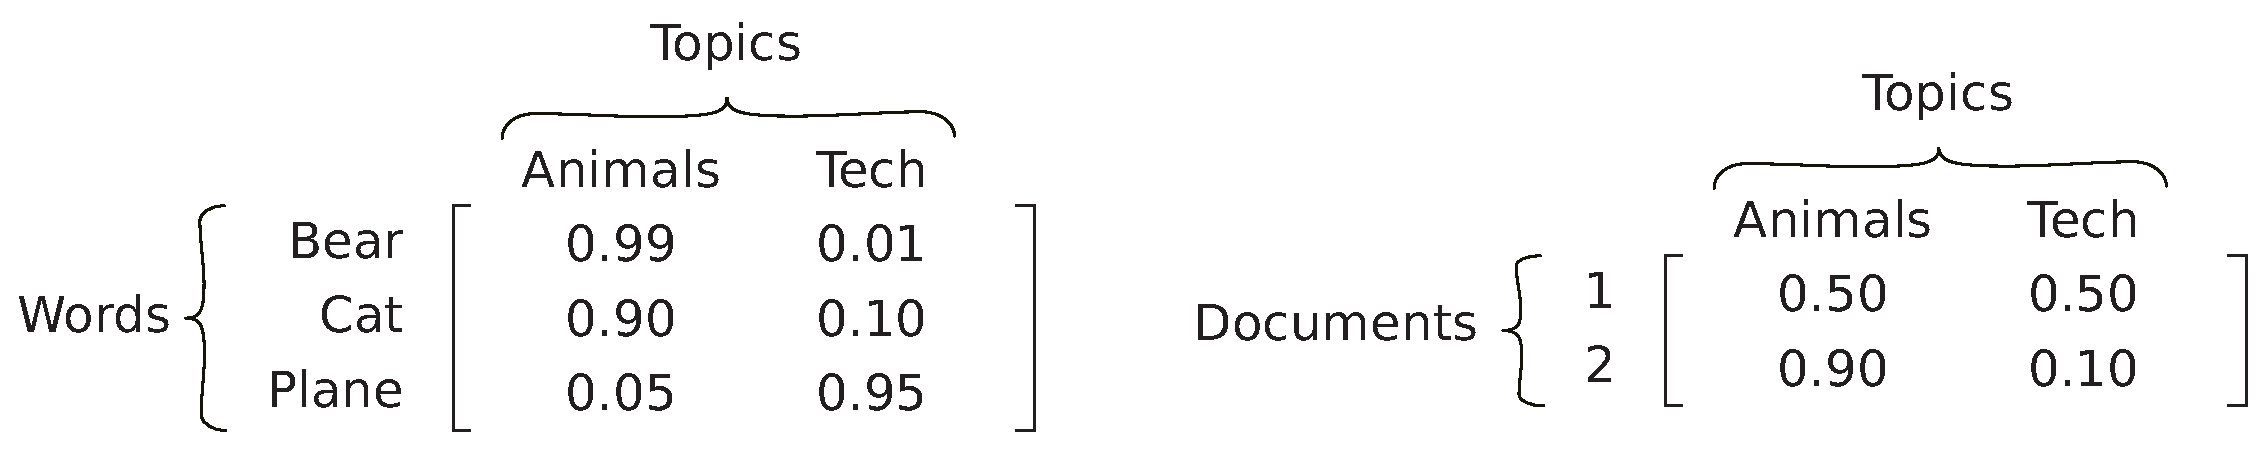
\includegraphics[width=\textwidth]{images/topic-mat.eps}}
    \caption{Example of a term-topic and a document-topic matrix.}
    \label{fig:topicmat}
\end{figure}

\section{Online LDA}
\dots

\section{Latent Dirichlet Allocation (LDA)}
\dots

\section{Hierarchical Dirichlet Process (HDA)}
\dots